\chapter{Сверхоперативная память --- кэши}\label{chapter11}

\dictum[Дональд Кнут. Искусство программирования. Сортировка и поиск]{Эта глава могла бы носить более претенциозное название --- <<Хранение и получение информации>>; с другой стороны, её можно было бы назвать кратко и просто --- <<Просмотр таблиц>>.}

\section{Стена памяти}

С развитием технологии микропроцессоры становились всё быстрее за счёт повышения тактовой частоты, увеличения ширины машинного слова и других факторов. В определённый момент было замечено, что все эти улучшения не дают существенного прироста скорости исполнения программ по той причине, что рост скорости оперативной памяти, используемой в ЭВМ, не столь стремителен. В результате процессор вынужден простаивать, ожидая, пока данные из памяти будут доставлены. Данная проблема получила название \textit{стены памяти} (\abbr memory wall, рис.~\ref{fig:mem-wall}) и означает, что в случае неизменности основных принципов организации вычислений рост производительности систем будущего ограничен именно скоростью оперативной памяти. 

\begin{figure}[htb]
    \centering
    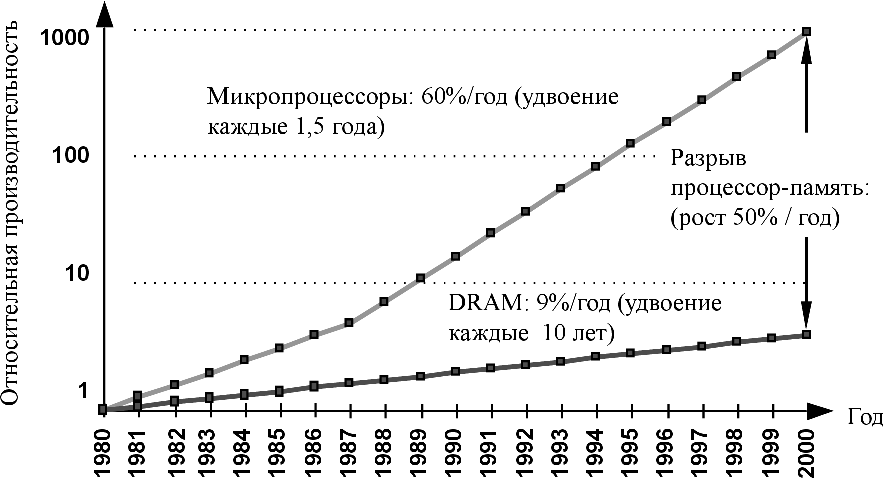
\includegraphics[width=0.85\textwidth]{./mem-wall-crop.pdf}
    \caption{Сравнительный рост скорости оперативной памяти и микропроцессоров}
    \label{fig:mem-wall}
\end{figure}

\section{Назначение, принцип работы}

Существует как минимум две области применения сверхоперативной памяти. Первая из них связана с описанной выше проблемой медленности доступа к ОЗУ. Вторая --- с обеспечением корректной и быстрой синхронизации работы многопроцессорных систем.

\subsection{Ускорение обращений в память}

Частично компенсировать данную проблему призваны устройства сверхоперативной памяти, в настоящее время чаще всего именуемые \textit{кэшами} (\abbr cache). Для большинства алгоритмов наблюдается выполнение принципов как временной, так  и пространственной  локальности: данные, к которым обращались недавно, скорее всего, будут запрошены снова в ближайшем будущем; кроме того, вероятно, что соседние с ними данные тоже будут запрошены (рис.~\ref{fig:locality}.). Представляется разумным иметь небольшое по сравнению с основной оперативной памятью хранилище, расположенное ближе к процессору и потому работающее быстрее, чтобы хранить в нём наиболее часто запрашиваемые данные. В кэше хранятся копии блоков информации, соответствующих подмножеству адресов оперативной памяти~\cite{ulrich-cpumemory, ulrich-cpumemory-rus}.

\begin{figure}[htb]
    \centering
    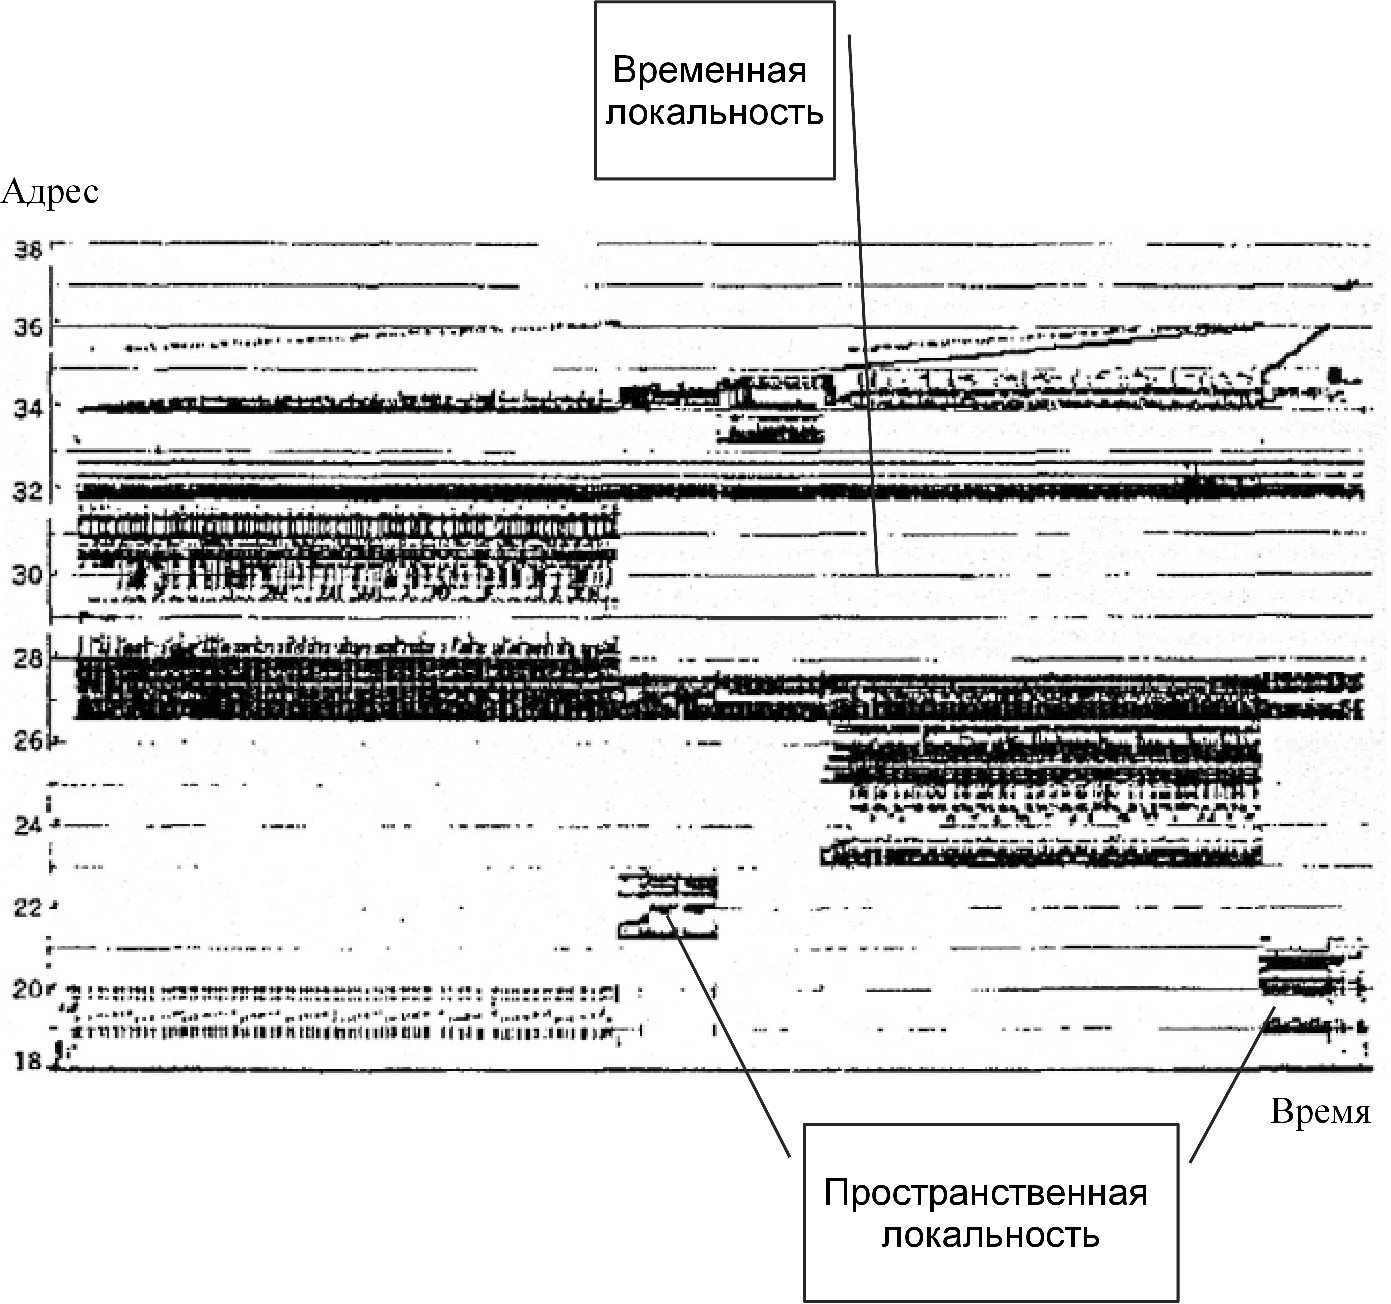
\includegraphics[width=0.80\textwidth]{./locality-crop.pdf}
    \caption[Пример явлений временной и пространственной локальности]{Пример явлений временной и пространственной локальности доступов памяти при работе приложения. Иллюстрация взята из~\cite{DBLP:journals/ibmsj/HatfieldG71}}
    \label{fig:locality}
\end{figure}


Данные в кэш попадают двумя способами. Во-первых, новый регион памяти может быть запрошен впервые за время работы, причем его придётся извлекать из основной памяти с задержкой, однако копия попадёт в кэш, и последующие обращения будут обработаны быстрее. Во-вторых, программист может предусмотреть, что некоторый диапазон памяти вскоре будет использован, и использовать явную \textit{предварительную загрузку} (\abbr prefetching) ещё до первого к нему обращения. Многие архитектуры имеют для этого специальные инструкции.

Поскольку ёмкость кэша невелика, а рабочее множество программы со временем меняется, неизбежно возникает ситуация, когда часть кэша придётся использовать для новых данных, а хранившийся там блок или отбросить, или, если он был изменён, записать обратно в память. Такой процесс называется \textit{вытеснение} (\abbr eviction).

Случаются ситуации, когда содержимое всего кэша перестаёт быть релевантным исполняемому коду. В таком случае происходит \textit{сброс} (\abbr flush) кэша, когда из него принудительно вытесняются все данные.

\subsection{Поддержка транзакций}
% \paragraph{Поддержка транзакций}

Использование дополнительного буфера в виде кэша позволяет откладывать момент записи в память, накопляя в нём совершённые последовательные изменения, применённые к различным адресам в памяти. Затем содержимое может быть записано за один раз, создавая видимость неделимости (атомарности) акта модификации ---  для внешнего наблюдателя памяти это будет выглядеть так, как будто сразу, без промежуточного состояния, изменилось большое число байт. Мы получаем транзакционную семантику записей в память. С другой стороны, если по каким-то причинам было решено, что все доступы в память, содержащиеся в кэше некоторого процессора, уже неактуальны, можно просто очистить его --- откатить транзакцию, и для внешнего наблюдателя это будет выглядеть так, как будто никаких операций над памятью не было выполнено.

Описанный  механизм является основным для реализации т.н. систем с аппаратной \textbf{транзакционной памятью}~\cite{rajwar2002}.

\begin{digression}

Акцент данной главы смещён от собственно сценариев/алгоритмов эмуляции к описанию архитектурных принципов работы самой сверхоперативной памяти. 

Первый сценарий применения систем кэшей подразумевает улучшение временных характеристик основного оперативного запоминающего устройства прозрачно для исполняющихся программ. Во многих функциональных моделях, пренебрегающих задержками, модели кэша может и не быть вовсе, несмотря на то, что в реальной аппаратуре он присутствует. Необходимость в его аккуратном моделировании возникает при  исследовании производительности подсистемы памяти.

Во втором случае влияние кэшей видимо на функциональном уровне и уже нельзя пренебрегать их функциональным моделированием. В наборе инструкций могут присутствовать команды управления транзакциями. Примером является расширение Intel\textregistered TSX~\cite[глава 8]{intel-x-reference}, ожидаемое в процессорах микроархитектуры Haswell.

\end{digression}


\section{Устройство кэша --- линии, тэги, ассоциативность}

Рассмотрим общий принцип организации кэша\footnote{Однако отметим, что описанная далее схема не является единственно возможной. Интересующийся читатель найдёт более полную картину в \cite{hennessy-patterson}.}. См. рис.~\ref{fig:cache}.

\begin{figure}[htb]
    \centering
    % \includegraphics[width=0.7\textwidth]{./cache-crop.pdf}
\begin{tikzpicture}[>=latex, font=\small]
    \draw[xstep=1cm, ystep=0.5cm] (0,0) grid (4,2);
    \draw[decorate, decoration={brace, amplitude=6pt}, xshift=-0.2cm]  (0,0) -- (0,2) node[midway, sloped, above=0.2cm] {$N_{sets}$};
    \draw[decorate, decoration={brace, amplitude=6pt}, yshift=0.2cm]  (0,2) -- (4,2) node[midway, sloped, above=0.2cm] {$N_{ways}$};
    \draw[very thick] (3,0) rectangle (4, 0.5);
    \node[draw, inner ysep=0pt, minimum height=.8cm] at (1, -1) (tag) {Тэг};
    \node[draw, inner ysep=0pt, minimum height=.8cm, right=0cm of tag, anchor=west] (flags) {Флаги};
    \node[draw, inner ysep=0pt, minimum height=.8cm, right=0cm of flags, anchor=west] (data) {Данные};
    \draw[dotted] (3,0) -- (tag.north west);
    \draw[dotted] (4,0) -- (data.north east);
\end{tikzpicture}
    \caption[Организация кэша в линии, сеты, пути]{Организация кэша в линии, сеты $N_{sets}$, пути $N_{ways}$. Ячейка содержит информацию: тэг, флаги и собственно данные линии}
    \label{fig:cache}
\end{figure}


Единица хранимых данных именуется \textit{линией кэша}. Как правило, она имеет ёмкость в несколько машинных слов и хранит копию последовательной области памяти, начиная с адреса, выровненного по размеру линии. В современных процессорах размер линии может быть 32 или 64 байта. 

Смысл кэша состоит в возможности быстрого нахождения соответствия «адрес--данные» (ситуация \textit{попадания в кэш}, \abbr cache hit) или констатации отсутствия такого соответствия (ситуация \textit{промаха}, \abbr cache miss). Алгоритм такого поиска состоит из следующих шагов.

\begin{enumerate*}
\item Каждая ячейка кэша кроме собственно копии данных содержит вспомогательную информацию, состоящую из тэга и группы флагов.

\item Из адреса в памяти выделяются смещение байта внутри линии \textit{offset}, номер множества (сета) $n_{set}$ и тэг $tag$. Пример такого разбиения приведён на рис.~\ref{fig:set-tag-flags}. Алгоритм выделения $n_{set}$ и $tag$ может быть произвольным, однако он должен позволять однозначно идентифицировать адрес линии.

\begin{figure}[htb]
    \centering
    % \includegraphics[width=0.35\textwidth]{./set-tag-flags-crop.pdf}
\begin{tikzpicture}[>=latex]
    
\begin{scope} [start chain,every node/.style={, font=\huge\ttfamily, text height=0.9cm}, node distance=0.cm,, inner sep=0cm]
    \node [on chain] (0x) {0x};
    \node [on chain] (set) {a};
    \node [on chain] {b};
    \node [on chain] {c};
    \node [on chain] {d};
    \node [on chain] {e};
    \node [on chain] {f};
    \node [on chain] (tag) {1};
    \node [on chain] {2};
    \node [on chain] {3};
    \node [on chain] {4};
    \node [on chain] {5};
    \node [on chain] {6};
    \node [on chain] (offset) {7};
    \node [on chain] {8};
    \node [on chain] {9};
    \node [on chain] (lastbit) {0};
\end{scope}

\draw (set.north west) -- ([yshift=-2cm] set.north west) coordinate[pos=0.95] (set-left) coordinate[pos=0] (bit63);
\draw (tag.north west) -- ([yshift=-2cm] tag.north west) coordinate[pos=0.95] (tag-left) coordinate[pos=0] (bit40-39);
\draw (offset.north west) -- ([yshift=-2cm] offset.north west) coordinate[pos=0.95] (offset-left) coordinate[pos=0] (bit16-15);
\draw (lastbit.north east) -- ([yshift=-2cm] lastbit.north east) coordinate[pos=0.95] (offset-right) coordinate[pos=0] (bit0);
    
\draw[<->] (set-left) -- (tag-left) node[midway, above] {\small номер сета};
\draw[<->] (tag-left) -- (offset-left) node[midway, above] {\small номер тэга};
\draw[<->] (offset-left) -- (offset-right) node[midway, above] {\small смещение};
    
\node at ([xshift=0.25cm] bit63) {\small 63};    
\node at (bit40-39) {\small 40 39};    
\node at (bit16-15) {\small 16 15};    
\node at ([xshift=-0.25cm] bit0) {\small 0};    
    
\end{tikzpicture}
    \caption[Пример выделения значений номера сета, тэга и смещения из адреса]{Пример выделения значений номера сета, тэга и смещения по диапазонам бит из адреса в шестнадцатеричном представлении}
    \label{fig:set-tag-flags}
\end{figure}


\item Выбирается сет с указанным $n_{set}$. Искомая линия может находиться в любом из $N_{ways}$ позиций в нём; ищется ячейка, содержащая тэг, равный $tag$. Аппаратная реализация большинства кэшей подразумевает, что поиск этот происходит параллельно во всех линиях сета и потому занимает фиксированное время.

\item Если удовлетворяющая условию ячейка найдена, проверяется, активна ли она или является «мусором», оставшимся от предыдущей работы.

\item В случае нахождения тэга и валидности мы имеем попадание в кэш, иначе же --- промах.
\end{enumerate*}

Таким образом, следующие параметры определяют описанный выше простой кэш.

\begin{itemize*}
\item Ёмкость линии данных $S_{line}$, измеряемая в байтах.
\item    Ассоциативность $N_{ways}$ определяет, сколькими способами одна и та же линия может быть размещена в ячейках кэша,  а также адреса линий, конкурирующих с ней за место (очевидно, что линии с разным значением $n_{set}$ всегда будут в разных сетах и не могут вытеснять друг друга). Если $N_{ways} = 1$, то мы имеем кэш \textit{прямого отображения} (\abbr directly mapped cache), в котором линия с определённым адресом, если она присутствует, всегда занимает одну и ту же ячейку. Соответственно, если $N_{sets} =1$, мы имеем полностью \textit{ассоциативный кэш} (\abbr fully associative cache), в котором линия может занимать любую ячейку.

\item    Количество сетов $N_{sets}$ должно быть достаточно большим, чтобы вместе с ёмкостью тэга быть способным полностью адресовать все возможные адреса линий в памяти системы. В противном случае некоторые диапазоны памяти просто не смогут быть отображены на ячейки.

\item    Ёмкость кэша --- $C$. Очевидно, что она равна произведению рассмотренных ранее величин:

$$C = S_{line}N_{ways} N_{sets}.$$
\end{itemize*}


\section{Промахи. Алгоритмы вытеснения линий}

Что должно происходить, если был детектирован промах кэша? Отсутствующие данные запрашиваются из памяти и, как правило, после получения помещаются в кэш. Для размещения новой линии может быть использована любая пустая, т.е. не содержащая актуальных данных, ячейка.

Как поступать, если все ячейки сета содержат актуальные данные? В таком случае выбирается одна из них, и её содержимое вытесняется и заменяется на новое. Перед этим проверяется ещё один флаг --- \textit{модификации} (\abbr dirty), поднимаемый при первой записи в ячейку. Если хранящиеся  в линии данные отличаются от версии, содержащейся в оперативной памяти, то необходимо передать их из кэша обратно в ОЗУ. Для ячеек, использовавшихся только для чтения, в этом нет необходимости, и они могут быть сразу перезаписаны.

Как выбрать, какую ячейку текущего сета следует вытеснить? «Идеальный» алгоритм --- выбирать линию с адресом, к которому впоследствии программа не будет обращаться дольше всего. Однако  его реализация подразумевает знание поведения алгоритма в будущем, а такой анализ в общем случае как минимум затруднителен, а с практической стороны и вовсе невозможен. Мы можем отталкиваться от истории предыдущих доступов к линиям при формулировке \textit{политики вытеснения} (\abbr replacement policy) линий.

Перечислим лишь некоторые из существующих алгоритмов~\cite{arc}.

\begin{itemize*}
\item    Вытеснять всегда первую ячейку. Очевидно, что это --- единственная доступная схема работы для кэша с прямым отображением. Для ассоциативных кэшей она нецелесообразна.

\item    Вытеснять случайную ячейку. Политика довольно проста в реализации, не требует хранения дополнительных данных для каждой ячейки, но может оказаться субоптимальной на практике.

\item    FIFO (\abbr first in first out) --- \textit{классическая очередь}. Для каждого сэта хранится порядок, в котором занимались его ячейки. Для вытеснения выбирается самая <<старая>> ячейка. Достоинство данной политики --- в простоте и небольших накладных расходах «в железе». Однако для наибольшей эффективности алгоритма необходимо, чтобы приложение, использующее память, имело потоковый характер чтения памяти, что далеко не всегда наблюдается на практике --- к некоторым ранее затребованным адресам оно может обращаться снова и снова с нерегулярными интервалами.

\item    LRU (\abbr least recently used). Для каждой ячейки хранится её «возраст» --- величина, пропорциональная времени, прошедшему с момента последнего к ней обращения. При вытеснении выбирается самая «старая» ячейка, т.к. к ней не обращались дольше всего и потому, возможно, не обратятся в ближайшем будущем. Данная политика (и её различные оптимизации) является самой популярной из-за наилучшего сочетания точности работы и сложности реализации.

\end{itemize*}

\section{Трансляция адресов и кэш}

В большинстве современных архитектур процессоры имеют поддержку виртуальной (в русской традиции называемой \textit{математической}) памяти для многозадачных режимов работы. При этом каждая программа, исполняющаяся на машине, видит собственное упрощённое адресное пространство, содержащее код и данные только её самой, и использует его вне зависимости от местоположения в физической, «настоящей» памяти. 

Поиск в кэше может происходить по физическому адресу, по виртуальному или даже по их комбинации. Схема разбиения адресов на тэг и номер сета может быть различная, но подразумевающая однозначное соответствие линий в памяти и ячеек кэша\footnote{В этой и последующих секциях данной главы часть текста по архитектуре кэшей адаптирована из русского и английского разделов Википедии: \url{http://ru.wikipedia.org/wiki/Кэш_процессора}.}.

Наличие виртуальной памяти требует от процессора проведения трансляции виртуальных  адресов, используемых программой, в физические адреса, соответствующие реальному местоположению в ОЗУ. При этом возникают следующие обстоятельства.

\begin{itemize*}
\item    \textit{Задержка.} Значение физического адреса будет готово только спустя некоторое время (несколько тактов) после запроса преобразования виртуального. Потому при обращении к кэшу только по физическим адресам мы будем вынуждены ожидать завершения процесса преобразования, если не используется специальное устройство для кэширования отображений виртуальных адресов --- буфер ассоциативной трансляции (\abbr TLB, translation look-aside buffer).

\item    \textit{Эффект наложения.} Несколько виртуальных адресов могут соответствовать одному физическому (\abbr aliasing). Поэтому требуется проверка, что только одна линия с данным физическим адресом находится в кэше в любой момент времени.
\end{itemize*}

По использованию виртуальной адресации кэши могут быть классифицированы следующим образом. 
\begin{enumerate*}
\item Physically indexed, physically tagged (PIPT) --- \textit{физически индексируемые и физически тегируемые}. Они просты и избегают проблем с наложением, но медленны, так как перед обращением в кэш требуется запрос физического адреса в TLB. Этот запрос может вызвать промах в TLB и дополнительное обращение в основную память перед тем как наличие данных будет проверено в кэше.

\item Virtually indexed, virtually tagged (VIVT) --- \textit{виртуально индексируемые и виртуально тегируемые.} И для тегирования, и для индекса используется виртуальный адрес, благодаря чему проверки наличия данных в кэше происходят быстрее, не требуя использования трансляции. Однако возникает проблема наложения, когда несколько виртуальных адресов соответствуют одному и тому же физическому. В этом случае данные будут дважды помещены в разные ячейки, что усложняет поддержку когерентности. Другой проблемой являются \textit{гомонимы} (\abbr homonyms)---  ситуации, когда в один и тот же виртуальный адрес (из разных пользовательских процессов) отображаются различные физические адреса. Невозможно различить их исключительно по виртуальному индексу. Возможные решения: сброс кэша при переключении между задачами (context switch), требование непересечения адресных пространств отдельных процессов, тегирование виртуальных адресов идентификатором адресного пространства, использование физических тегов.

\item Virtually indexed, physically tagged (VIPT) --- \textit{виртуально индексируемые и физически тегируемые.} Для индекса используется виртуальный адрес, а для тега --- физический. Преимуществом над первым типом является меньшая задержка, поскольку можно искать кэш-линию одновременно с трансляцией адресов в TLB, однако сравнение тега всё равно задерживается до момента получения физического адреса. Преимуществом над вторым типом является безопасное обнаружение гомонимов, так как тег содержит физический адрес. Для данного типа требуется выделять больше бит для хранения тега, поскольку индексные биты используют иной тип адресации.

\item Physically indexed, virtually tagged --- \textit{физически индексируемые и виртуально тегируемые}. Такие кэши не дают существенных преимуществ и в настоящее время представляют исключительно академический интерес.
\end{enumerate*}

\section{Иерархии кэшей}

\subsection{Многоуровневые системы}

Может показаться очевидным, что чем больше ёмкость установленного кэша, тем эффективнее будет работать подсистема памяти из-за меньшей частоты промахов, необходимости вытеснения линий в ассоциативных сетах. Однако на практике эта величина ограничена многими факторами, в первую очередь доступной площадью на кристалле и энерговыделением. Кроме того, увеличение количества линий ведёт к росту геометрических размеров кристалла, время, затрачиваемое на передачу сигналов, растёт, нивелируя эффект от большего количества данных.

Невозможность улучшать уже присутствующие в системе устройства приводит к необходимости введения ещё одного промежуточного хранилища между ядром процессора и ОЗУ --- кэш второго уровня (L2). Он располагается сразу после кэша первого уровня (L1) и характеризуется большими задержками доступа, но при этом может иметь большую ёмкость, см. рис.~\ref{fig:l1l2}.

\begin{figure}[htb]
    \centering
    % \includegraphics[width=0.5\textwidth]{./l1l2-crop.pdf}
\begin{tikzpicture}[>=latex, font=\small]
\node[draw, circle, inner sep=1pt] (cpu) {ЦПУ};
\node[draw, text width = 2cm, align=center, below = 0.5cm of cpu] (l1) {L1};
\node[draw, text width = 4cm, align=center, below of=l1] (l2) {L2};
\node[draw, text width = 6cm, align=center, below of=l2] (ram) {ОЗУ};

\draw[<->] (cpu) -- (l1);
\draw[<->] (l1) -- (l2);
\draw[<->] (l2) -- (ram);

\end{tikzpicture}
    \caption{Иерархия памяти, состоящая из двух кэшей и ОЗУ}
    \label{fig:l1l2}
\end{figure}


Теперь при ситуации промаха в кэше первого уровня данные сначала ищутся во втором уровне, и лишь при втором промахе обращение идёт в память. 

Естественно, что иерархию памяти можно продолжать наращивать, добавляя новые, менее быстрые и более ёмкие уровни сверхоперативной памяти. %В большинстве современных процессоров имеется трёхуровневая система кэшей.

Для таких систем возникают следующие вопросы проектирования: на каких уровнях системы должна содержаться линия с определённым адресом при различных историях обращений к ней? Может ли одна линия находиться одновременно в нескольких уровнях кэша?

В одном случае могут потребовать, чтобы все данные, хранящиеся в кэше L1, находились также и в кэше L2. Такие пары кэшей называют строго \textit{инклюзивными} (\abbr inclusive). Другие процессоры могут не иметь подобного требования, тогда кэши называются \textit{эксклюзивными} (\textit{исключительными})  --- данные могут быть либо в L1, либо в L2 кэше, но никогда не могут быть одновременно в обоих.

До сих пор другим процессорам не требовалось, чтобы данные в кэше первого уровня также размещались в кэше второго уровня, тем не менее они продолжают так делать. Нет общепринятого имени для этой промежуточной политики, хотя часто используется термин \textit{инклюзивно} (\abbr mainly inclusive).

\subsection{Кэши инструкций и данных}

Инструкции, как и данные, хранятся в общем пространстве памяти\footnote{Для ЭВМ архитектуры фон Неймана; тем не менее дальнейшие рассуждения в основном применимы и для систем с гарвардской архитектурой.}; как и в случае данных, быстрый доступ к ним является необходимым условием скорости исполнения приложений. Однако множества используемых адресов и характерные шаблоны доступов для кода и данных чаще всего различны, что при их совместном кэшировании создало бы чрезмерную нагрузку и неоптимальное использование ресурсов сверх\-опера\-тивной памяти. Поэтому отдельно выделяют кэш инструкций (\abbr instruction cache, IC) и кэш данных (\abbr data cache, DC). Отметим, что в IC приходят только запросы на чтение. При работе такой системы нужно следить за тем, чтобы запись в DC по адресам линий, находящихся в IC, приводила к их сбросу\footnote{В некоторых архитектурах для этого следует явно вызывать инструкцию, в остальных происходит автоматически.}.

\section{Кэши в многопроцессорных системах}

В современных ЭВМ доступ к памяти могут одновременно иметь как несколько независимых процессоров (в многоядерных системах), так и ряд периферийных устройств (в системах с DMA --- \abbr direct memory access). Каждый из них может иметь свои приватные кэши, в которых хранятся копии линий, в том числе и локально модифицированных.  Необходимо, чтобы все агенты имели единое представление о содержимом ОЗУ. Кроме того, на производительность иерархии памяти, связанной с одним ядром, влияет то, как линии переходят между разными его уровнями.

\subsection[Классификация моделей согласованности]{Классификация моделей согласованности доступов в память}


Модель согласованности (консистентности) представляет собой некоторый договор между программами и памятью, в котором указывается, что работа модуля памяти будет корректной при соблюдении программами определённых правил. Существует их общепринятая алгоритмическая классификация~\cite{Mosberger93memoryconsistency}, основанная на различии тех моментов, когда транзакция становится видимой для сторонних наблюдателей, а также разрешённого порядка записи. Ниже перечислены лишь некоторые существующие модели.

\begin{enumerate*}
\item    \textit{Строгая согласованность.} Операция <<чтение ячейки памяти с адресом $x$>> должна возвращать значение, записанное самой последней операцией <<запись>> с адресом $x$. В системе со строгой консистентностью должно присутствовать единое абсолютное время.

\item    \textit{Последовательная согласованность} --- модель, в которой результат выполнения должен быть тот же, как если бы инструкции операторов всех процессов выполнялись в некоторой последовательности, определяемой программой для этого процессора. При параллельном выполнении все процессы должны видеть одну и ту же последовательность записей в память, то есть разрешаются запаздывания для чтения.

\item    \textit{Причинная согласованность} --- модель, не требующая, чтобы все процессы видели одну и ту же последовательность записей в память. Таким образом, проводится различие между потенциально-зависимыми (запись одной может зависеть от результата чтения другой ячейки) и потенциально-независимыми (параллельными) операциями записи.

\end{enumerate*}

На практике модели согласованности выражаются политиками записи в память, реализуемыми аппаратурой сверх- и оперативной памяти.

\subsection[Политики записи]{Политики записи: WT, WB, WC, UC}

При записи данных в кэш должен существовать определенный момент времени, когда они будут записаны в основную память, что контролируется \textit{политикой записи} (\abbr write policy). Для кэшей с политикой \textit{сквозной записи} (WT, \abbr write through) любая запись приводит к немедленной записи в память, происходящей параллельно с записью в ячейку кэша. 

Другая политика, именуемая \textit{обратной записью} (WB, \abbr write back), откладывает запись на более позднее время, которая производится при вытеснении подобной линейки из кэша. Таким образом, промах в кэше, использующем политику обратной записи, может потребовать двух операций доступа в память --- один для сброса состояния старой линейки и другой для чтения новых данных.

Режим \textit{совмещения записи} (WC, \abbr write combining) позволяет сохранять данные перед записью из кэша в память в специальном буфере, сбрасываемом за одну операцию, --- \textit{всплеск} (\abbr burst), вместо того, чтобы  писать эти линии немедленно по их прибытии, что приводит к повышению средней скорости записи. %\footnote{Фактически здесь мы видим подтверждение закона Литтла (см. главу~\ref{chapter06}).}.

Такой режим не следует использовать для доступа к «обычной» памяти кода и данных в силу её модели \textit{слабой согласованности} (\abbr weak ordering), которая не гарантирует, что последовательность записей и чтений будет выполнена в ожидаемом порядке. Например, комбинация «запись---чтение---запись» некоторого адреса при совмещённой записи выльется в последовательность «чтение---запись---запись», т.к. при чтении будет получено значение, хранящееся в памяти, а не в буфере. Для решения этой проблемы буфер может быть дополнен функциональностью полностью ассоциативного кэша --- дополнительного уровня в иерархии, что приведёт к усложнению его реализации.

Однако для видеопамяти слабая согласованность не является препятствием, и поэтому политика WC может быть использована для реализации быстрых драйверов видеокарт~\cite{wc-guidelines}.

В реальных системах различные диапазоны памяти могут иметь различные типы политик записи в память, настраиваемых с помощью атрибутов страниц ОЗУ или специальных системных регистров. В качестве одного из возможных типов может быть выбран полный \textit{запрет кэширования} (UC, \abbr uncacheable) --- такой режим необходим для регионов, соответствующих периферийным устройствам, доступ к которым вызывает немедленные побочные эффекты.

\subsection[Алгоритмы поддержания когерентности]{Алгоритмы поддержания когерентности}

Для того чтобы информация о состояниях линий в независимых кэшах соответствовала выбранной модели согласованности, используются специальные протоколы когерентности. Каждая ячейка кэша получает расширенный набор флагов, описывающий то, как её состояние соотносится с состояниями ячеек с тем же адресом, но находящихся в кэшах других агентов.

При изменении состояния некоторой линии необходимо каким-то образом сообщать о таком факте остальным кэшам. Генерируются сообщения, доставляемые по какой-либо среде внутри многопроцессорной системы (это может быть общая шина, полностью связанная сеть или сеть общего вида; сообщения могут быть адресными или широковещательными), и связанная с указанным фактом задержка влияет на скорость работы подсистемы памяти.

Было придумано много вариантов протоколов когерентности, отличающихся алгоритмами и количеством состояний, которые различаются по своей скорости работы и масштабируемости. Большинство современных протоколов представляют вариации т.н. MESI-протокола\footnote{Хороший обзор существующих протоколов с диаграммами переходов можно найти по ссылке \url{http://pg-server.csc.ncsu.edu/mediawiki/index.php/CSC/ECE_506_Spring_2011/ch8_mc}.}.

\subsubsection{MESI}

В этой схеме каждая линия имеет одно из взаимоисключающих состояний.

\begin{itemize*}
\item    \textit{Модифицированная} (\textit{M}) \abbr modified: данные в кэш-линии, помеченной как модифицированная, имеются только в одном кэше во всей системе. Линия может читаться и быть записана без опроса остальных агентов в системе.

\item    \textit{Исключительная} ( \textit{эксклюзивная} ) (\textit{E}) \abbr exclusive: кэш-линия, как и \textit{M}-линия, хранится только в одном кэше системы, однако она ещё не подверглась изменениям; данные в ней идентичны хранящимся в ОЗУ. Поскольку эксклюзивная кэш-строка хранится только в одной кэш-памяти, она может быть считана или записана без внешних запросов. После записи в линию она отмечается как модифицированная.

\item    \textit{Разделяемая} (\textit{S}) \abbr shared: линия может одновременно находиться в нес\-коль\-ких кэшах и использоваться совместно двумя или более агентами. Запросы на запись к такой линии  всегда идут на внешнюю шину данных независимо от политики записи (WT или WB) , что приводит линии в других кэшах в состояние «недействительно». При этом содержимое основной памяти также обновляется.

\item    \textit{Недействительная} (\textit{I}) \abbr invalid: линия, отмеченная как недействительная, становится логически недоступной. Это происходит в случаях, если она пуста или содержит устаревшую информацию. 

\end{itemize*}
Схема переходов представлена на рис.~\ref{fig:mesi}.

\subsubsection{MOESI}

Данный протокол является оптимизацией  обычного протокола MESI. При этом флаги состояния расширяются состоянием \textit{O} (\abbr owned), означающим, что данные в линии одновременно и модифицированы, и разделяются (modified и shared). Указанное состояние позволяет избежать необходимости записи модифицированной линии обратно в основную память, прежде чем другие процессоры системы смогут ее прочесть. Используется микропроцессорами AMD Opteron.
\begin{itemize*}
\item    \textit{Владелец} (Owned). Кэш-линия в этом состоянии содержит наиболее свежие, корректные данные. Описанное состояние похоже на Shared в том, что оно обозначает, что другие процессоры могут иметь копию наиболее свежих и корректных данных. Однако, в отличие от него, оно также обозначает, что в основной памяти данные могут быть устаревшими. Только один из агентов может иметь данную линию в состоянии Owned, вместе с тем он отвечает на запросы о чтении вместо памяти, с помощью этого ускоряя работу остальных агентов.
\end{itemize*}

\begin{figure}[htb]
    \centering
%     \includegraphics[width=0.7\textwidth]{./mesi-crop.pdf}
\begin{tikzpicture}[>=latex, node distance=3cm, font=\small]
    \node[circle, draw, minimum width=2cm] (invalid) {Invalid};
    \node[circle, draw, minimum width=2cm, right of=invalid] (exclusive) {Exclusive};
    \node[circle, draw, minimum width=2cm, below of=invalid] (modified) {Modified};
    \node[circle, draw, minimum width=2cm, right of=modified] (shared) {Shared};
    
\begin{scope}[node distance=0.6cm,font=\footnotesize]
    \node[right=1.5cm of exclusive.north] (local-read) {Местное чтение};
    \node[below=of local-read] (local-write) {Местная запись};
    \node[below=of local-write] (remote-read) {Удалённое чтение};
    \node[below=of remote-read] (remote-write) {Удалённая запись};
\end{scope}

\draw[->, dashdotted] ([yshift=-0.25cm] local-read.west) -- ([yshift=-0.25cm] local-read.east);
\draw[->, ] ([yshift=-0.25cm] local-write.west) -- ([yshift=-0.25cm] local-write.east);
\draw[->, dotted] ([yshift=-0.25cm] remote-read.west) -- ([yshift=-0.25cm] remote-read.east);
\draw[->, dashed] ([yshift=-0.25cm] remote-write.west) -- ([yshift=-0.25cm] remote-write.east);

\draw[->, dashdotted] (invalid) -- (exclusive);
\draw[->, dashdotted] (exclusive.0) .. controls +(1,0) and +(0,1) .. (exclusive.90);
\draw[->, dashdotted] (modified.180) .. controls +(-1,0) and +(0,-1) .. (modified.270);
\draw[->, dashdotted] (shared.270) .. controls +(0,-1) and +(1,0) .. (shared.0);

\draw[->] (invalid) -- (modified);
\draw[->] (exclusive.205) .. controls +(-1,0) and +(1,0) .. (modified.45);
\draw[->] (shared.205) -- (modified.335);
\draw[->] (modified.270) .. controls +(0,-2) and +(-2,0) .. (modified.180);

\draw[->, dotted] (exclusive) -- (shared);
\draw[->, dotted] (modified) -- (shared);
\draw[->, dotted] (shared.0) .. controls +(2,0) and +(0,-2) .. (shared.270);

\draw[->, dashed] (exclusive.135) -- (invalid.45);
\draw[->, dashed] (modified.135) -- (invalid.225);
\draw[->, dashed] (shared.125) .. controls +(-1,0) and +(1,0) .. (invalid.315);
\end{tikzpicture}

    \caption[Диаграмма переходов протокола MESI]{Диаграмма переходов протокола MESI. Доступ является местным, если он был инициирован процессором данного кэша, и удалённым, если запрос возник в любом другом}
    \label{fig:mesi}
\end{figure}

\subsubsection{MESIF}

Данный протокол актуален для систем с неоднородной когерентной памятью (\abbr cache coherent non-uniform memory access, ccNUMA), когда каждый процессорный сокет имеет свою, ближайшую к нему, память, а обращение к адресам других сокетов происходит через промежуточные узлы и занимает в 1,5---2 раза больше времени. Введение к протоколу MESI нового состояния \textit{F} (\abbr forward) сделано для уменьшения объёма синхронизационного траффика в таких системах; фактически \textit{F} --- это вариант \textit{S}, присутствующий ровно в одном кэше в любой момент времени.
\begin{itemize*}
\item \textit{Передовой} (\textit{F}): означает, что данный кэш является единственным выбранным ответчиком (\abbr designated responder) для любых запросов к линии с данным адресом. Остальные линии (в состоянии \textit{S}) при этом не отвечают на запросы когерентности. 
\end{itemize*}

\section{Моделирование}

При симуляции систем кэшей количество необходимых усилий напрямую зависит от реализуемой архитектуры и сценария использования этой модели.

\subsection{«Честное» моделирование}

Зачастую модель кэша повторяет устройство реальной аппаратуры очень близко для того, чтобы учесть все возможные причины возникновения задержек. При этом функционально моделируется хранение в ячейке данных, метаданных (тэги, флаги, информация для механизма вытеснения). Для иерархий кэшей учитываются передачи данных между уровнями. Для когерентных систем приходится добавлять модель среды для передачи данных и симулировать полную маршрутизацию сообщений от одних кэшей до других.

Отметим, что механизм ассоциативного поиска тэга внутри сета нереализуем программно (по крайне мере в одном потоке исполнения), и потому он заменяется более традиционными алгоритмами --- последовательный перебор, деревья, хэш-таблицы; величина задержки этой процедуры, конечно, учитывается вне зависимости от деталей модельной реализации.

\subsection{Модель задержек}

Этот подход применим в том случае, когда кэши функционально «прозрачны» и их наличие выражается только в изменении времён доступов к памяти. В таком случае мы можем упростить их моделирование,  избавившись от хранения линий --- они всегда будут лежать в устройстве памяти, кэш не будет содержать их копии. Для вычисления же времён задержек все метаданные (тэги, сеты, флаги) ячеек моделируются так же, как и в общем случае.

Для моделирования аспектов задержки доступов, связанной с необходимостью передачи данных для поддержания когерентности, может быть использована более простая схема, отражающая функциональность, но не детали её реализации; при этом время высчитывается по заранее измеренным «расстояниям» между агентами (рис.~\ref{fig:timing-model}). Такое разделение упрощает разработку модели кэшей и ускоряет исследование различных её вариантов. Однако оно неприменимо для случая моделирования транзакций, так как фактически данные никуда не перемещаются и их копии не создаются.

\begin{figure}[htb]
    \centering
%     \includegraphics[width=0.6\textwidth]{./timing-model-crop.pdf}
\begin{tikzpicture}[>=latex, font=\small]
    % FIXME the whole drawing is done awfully
    \draw (0,0) rectangle (3,1.5);
    \node[text width = 3cm, anchor=north west, font=\footnotesize] at (0,1.5)  {Функциональная модель ОЗУ};
    \path (1.5, 0.25) coordinate (c1) -- (2.0,0.5) coordinate (d1);
    \node[draw, inner sep=0pt, fit=(c1) (d1)] (func-cell) {};
    
    \draw (3.999,0) coordinate (e1) grid[xstep=0.5, ystep=0.25] (7,1.5) coordinate (f1);
    \path (e1) -- (f1) coordinate[pos=0.5] (cache-middle);
    \node[fill=white] at (cache-middle) {Модель кэшей};
    
    \path (5.5, 0.25) coordinate (w1) -- (6,0.5) coordinate (z1);
    \node[inner sep=0pt, fit=(w1) (z1)] (time-cell) {};
    
    \path (0,-1.8) coordinate (a1) rectangle (7,-1.) coordinate (b2);
    \node[draw, align=center, inner sep=0pt, fit=(a1) (b2)] (dev) {Процессор};
    
    % The coordinates addressing is really stupid here
    \draw[->] ([xshift=-2.5cm] dev.north) -- ([xshift=-2.5cm, yshift=1cm] dev.north) node[midway, above, sloped, font=\scriptsize] {Адрес};
    \draw[->] (func-cell.south) -- ([yshift=-1.25cm] func-cell.south) node[yshift=2pt,fill=white, inner sep=0pt, midway, above, sloped, font=\scriptsize] {Данные};

    \draw[->] ([xshift=1.5cm] dev.north) -- ([xshift=1.5cm, yshift=1cm] dev.north) node[midway, above, sloped, font=\scriptsize] {Адрес};
    

    \draw[->] (time-cell.south) -- ([yshift=-1.25cm] time-cell.south) node[yshift=2pt, fill=white, inner sep=0pt, midway, above, sloped, font=\scriptsize] {Задержка};

\end{tikzpicture}
    \caption[Раздельное моделирование функциональности и длительности доступов в~память]{Раздельное моделирование функциональности и длительности доступов в память. По указанному адресу данные возвращаются моделью памяти (кэши при этом не оказывают никакого влияния), задержки независимо вычисляются моделью кэшей}
    \label{fig:timing-model}
\end{figure}

\subsection[Влияние моделей кэшей на скорость]{Влияние моделей кэшей на скорость симуляции}

Подключение системы кэшей к функциональной модели делает её (хотя бы частично) потактовой, и естественно ожидать связанное с этим замедление симуляции. На практике скорость может упасть в тысячи раз. Поэтому часто модели кэши делают динамически отсоединяемыми от иерархии памяти, и они подключены лишь на период симуляции, когда исполняется изучаемое приложение, чтобы не тормозить предваряющие этапы загрузки операционной системы. 

Однако очевидно, что эффективность кэша будет зависеть от того, заполнен ли он актуальными данными или же пуст; во втором случае многие ранние доступы будут промахами. Поэтому после подключения некоторое время тратится на \textit{разогрев} (\abbr warm up) системы, причем статистика и задержки игнорируются (рис.~\ref{fig:warm-up}). Длительность этого процесса зависит от ёмкости кэшей и интенсивности обращений приложения к памяти; как минимум длина его не должна быть меньше длины периода измерения. Лишь после разогрева появляются основания полагать, что измеряемые на модели результаты производительности будут адекватны реальности. 

\begin{figure}[htb]
    \centering
%     \includegraphics[width=0.9\textwidth]{./warm-up-crop.pdf}
\begin{tikzpicture}[font=\scriptsize, >=latex, shape=signal, signal from=west, text width=2.5cm, minimum height=1.5cm, signal pointer angle=120, inner sep=2pt]
    \node[draw,] (boot-os) {Загрузка ОС. Кэши отключены. Измерения не производятся.};
    \node[draw, right=0cm of boot-os] (warmup) {Изучаемое приложение. Кэши включены. Измерения не производятся.};
    \node[draw, right=0cm of warmup] (measure) {Изучаемое приложение. Кэши включены. \textbf{Проводятся измерения}.};
\end{tikzpicture}
    \caption[Разогрев кэшей]{<<Разогрев>> кэшей. Этап симуляции загрузки ОС проводится с помощью быстрой функциональной модели. Затем некоторое время система кэшей подключена и обрабатывает запросы, но статистика и сообщаемые ей задержки не принимаются во внимание. На последнем отрезке собираются результаты моделирования}
    \label{fig:warm-up}
\end{figure}

\iftoggle{hasquiz}{
    \section{\Questions к главе \ref{chapter11}} %\label{chapter11-questions}

\subsection*{Вариант 1}

\begin{questions}
\question[3] Выберите правильные варианты продолжения фразы: использование кэшей при работе приложения целесообразно, если
\begin{choices}
    \correctchoice    программа показывает временную локальность доступов,
    \choice программа не обращается в оперативную память,
    \choice программа работает с очень большим объёмом данных,
    \correctchoice программа показывает пространственную локальность доступов,
    \choice программа работает с объёмом данных, меньшим ёмкости кэша.
\end{choices}

\question[3] Выберите все правильные окончания фразы: функциональные симуляторы часто не содержат в себе модель кэша, потому что
\begin{choices}
    \correctchoice они влияют только на задержки, но не на семантику инструкций,
    \choice всегда имеется возможность переиспользовать хозяйский кэш для нужд симуляции,
    \correctchoice такие модели сильно замедляют симуляцию.
\end{choices}

\question[3] Данные могут попадать в кэш при следующих операциях:
\begin{choices}
    \correctchoice чтение памяти (load),
    \correctchoice запись в память (store),
    \choice арифметические операции,
    \choice операции с числами с плавающей запятой,
    \correctchoice предвыборка данных (prefetch),
    \correctchoice загрузка инструкции (fetch),
    \choice инвалидация линии (invalidate).
\end{choices}

\end{questions}

\subsection*{Вариант 2}
\begin{questions}

\question[3] Выберите правильные варианты окончания: линия данных с фикированным адресом
\begin{choices}
    \choice всегда попадает в одну и ту же ячейку кэша,
    \correctchoice всегда попадает в один и тот же сет,
    \choice может быть сохранён в любой ячейке кэша.
\end{choices}

\question[3] Выберите правильные варианты.
\begin{choices}
    \choice Темпы роста скорости оперативной памяти и процессоров одинаковы с 80-х годов ХХ века.
    \choice Темп роста скорости оперативной памяти опережает темпы роста скорости работы процессоров.
    \correctchoice Темп роста скорости процессоров опережает темпы роста скорости оперативной памяти. 
\end{choices}

\question[3] Кэши необходимо симулировать даже в функциональной модели, если они используются для
\begin{choices}
    \correctchoice создания транзакционной памяти,
    \choice моделирования работы ЭВМ гарвардской архитектуры,
    \choice поддержания когерентности в SMP системах.
\end{choices}





\end{questions}

% К каждой лекции должно быть от 8 до 12 задач, у каждой задачи должно быть 3-5 вариантов формулировок примерно одинаковой сложности. Допускается объединение нескольких последовательных лекций в одну тему и подготовка тестов к темам.
% Задачи должны полностью соответствовать материалам лекций, то есть лекциях должно быть достаточно информации для ответа на все вопросы.
% Формулировка каждого варианта задачи должна содержать всю необходимую информацию и не должна ссылаться на тексты внутри лекции, картинки или другие задачи или варианты задачи.
% Правильные ответы выделяются знаком «+» перед их формулировкой. Правильных ответов может быть несколько. Для тестов с несколькими ответами как минимум один ответ должен быть правильным и как минимум один ответ должен быть неправильным. 
% 
% Структура теста к лекции
% 
% \subsection*{Задача 1}
% 
% \paragraph{Вариант 1} 
% 
%     Чему равно 2+2?
%         Ответ 1. 3
%         + Ответ 2. 4
%         …
%         Ответ N. 5
% \paragraph{Вариант 2}
%     Чему равно 2*2?
%         + Ответ 1. 4
%         + Ответ 2. 2+2
%         …
%         Ответ N. 5
% \paragraph{Вариант 3}
% 
%     Чему равно 2-2?
%         Ответ 1. 0
% 
% 
%         
% \section{Просто подборка вопросов}
% 


 
 
}{}


\iftoggle{webpaper}{
    \printbibliography[title={Литература}]
}{}

